\begin{figure}[!h]
	\begin{minipage}[b]{0.49\linewidth}
		\centering
		\centerline{ 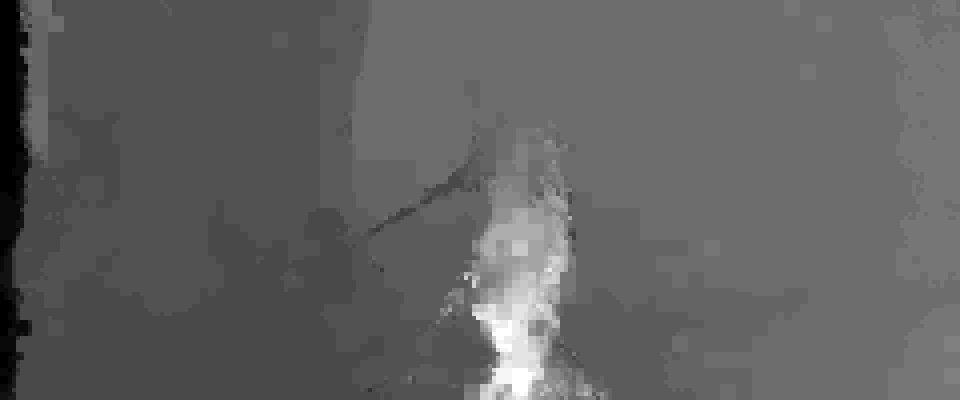
\includegraphics[width=\linewidth]{motionx} }
		\centerline{\scriptsize{(a) Horizontal-motion strength map}}\medskip
	\end{minipage}%
	\hfill
	\begin{minipage}[b]{0.49\linewidth}
		\centering
		\centerline{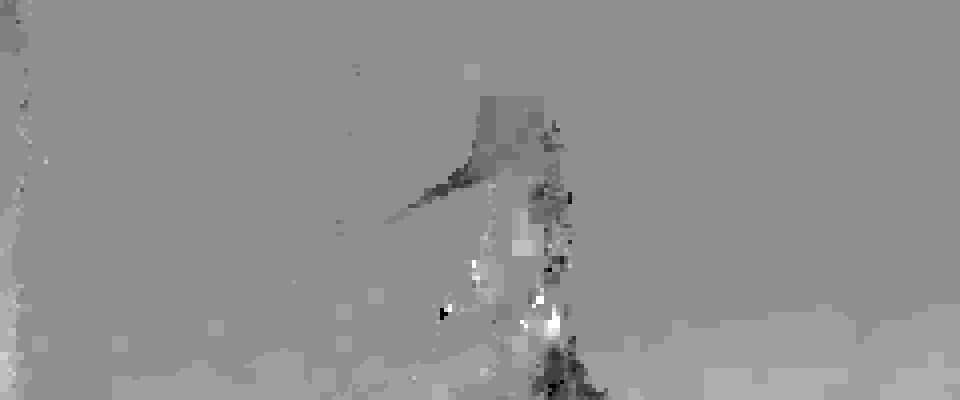
\includegraphics[width=\linewidth]{motiony} }
		\centerline{\scriptsize{(b) Vertical-motion strength map}}\medskip
	\end{minipage}
	\begin{minipage}[b]{0.49\linewidth}
		\centering
		\centerline{ 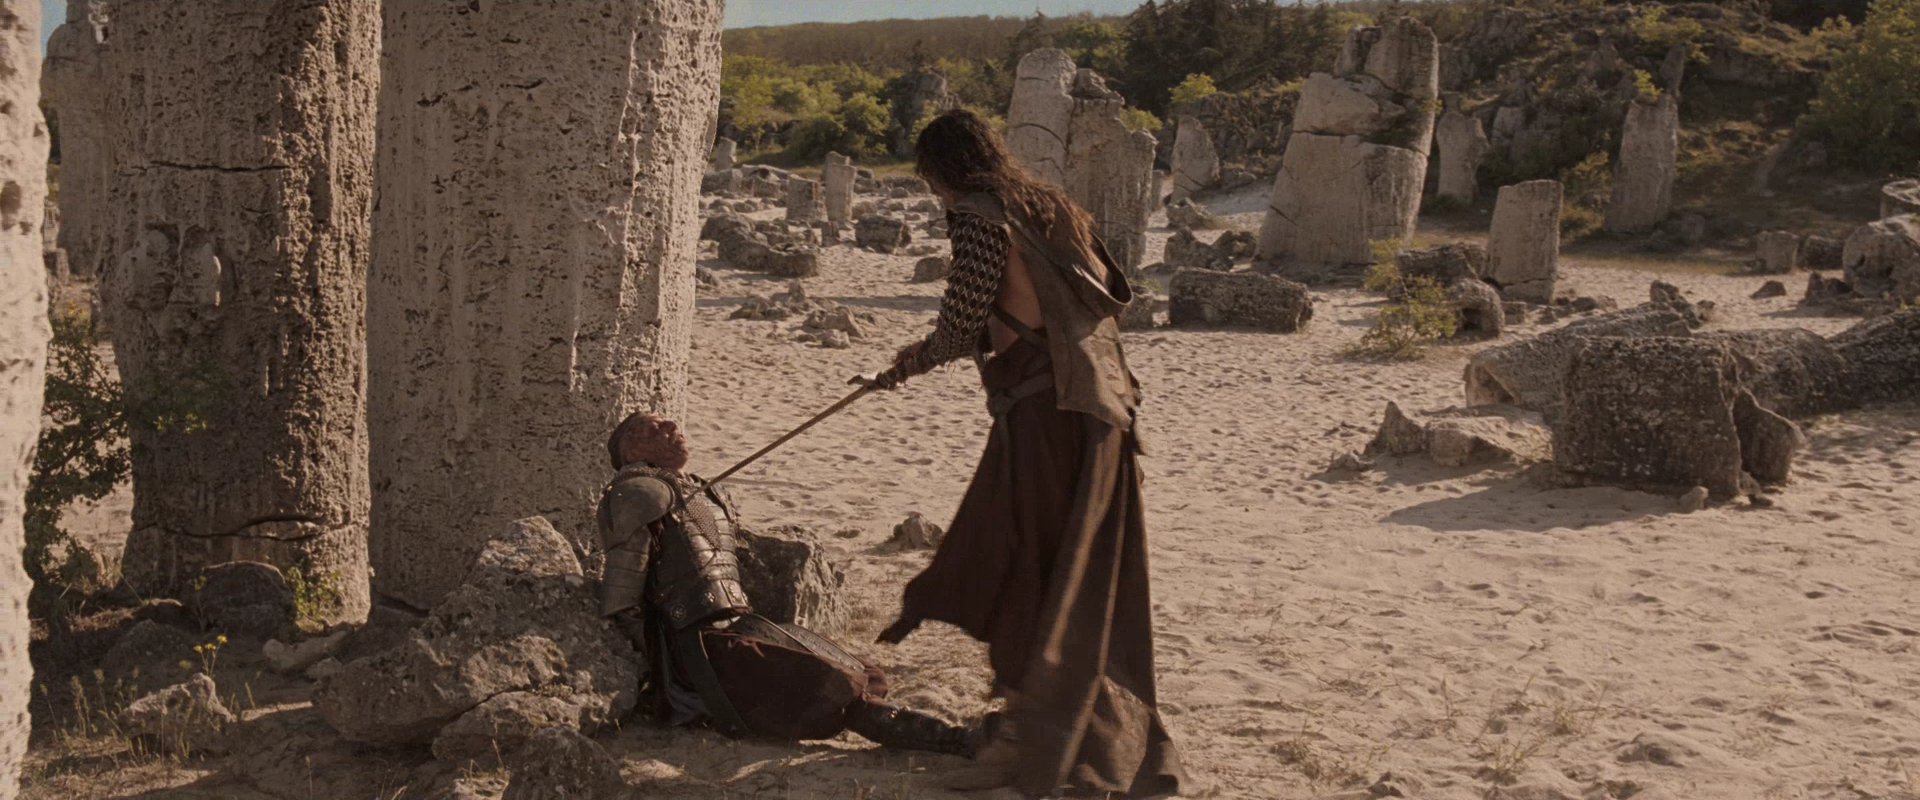
\includegraphics[width=\linewidth]{src} }
		\centerline{\scriptsize{(c) Source left view}}\medskip
	\end{minipage}%
	\hfill
	\begin{minipage}[b]{0.49\linewidth}
		\centering
		\centerline{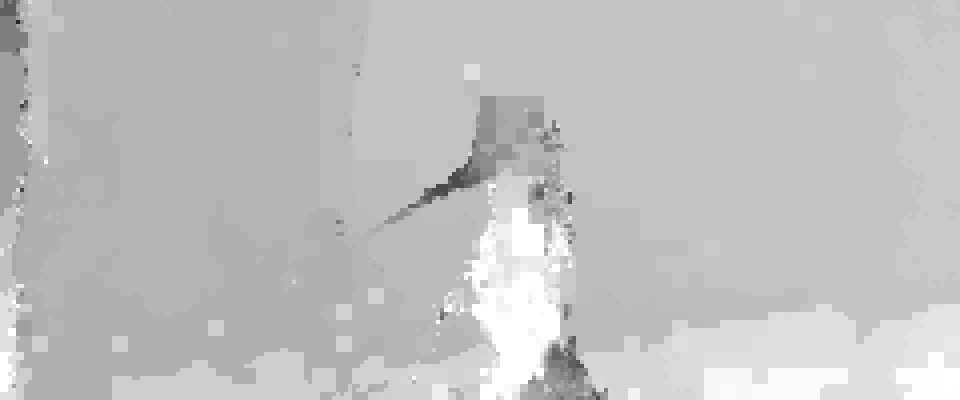
\includegraphics[width=\linewidth]{merged} }
		\centerline{\scriptsize{(d) Overall motion-strength map}}\medskip
	\end{minipage}
	\begin{minipage}[b]{\linewidth}
	\caption{Example maps of horizontal~(a) and vertical~(b) motion extracted
        using a block-based motion-estimation algorithm~\cite{simonyan2008fast} for the source frame~(c).
        The results  are combined into an overall motion-strength map~(d).}
    \label{fig:merged}
    \end{minipage}
\end{figure}
